%% Time-stamp: <2019-01-22 14:47:04 (marc)>
\documentclass[xcolor=x11names,compress, mathserif]{beamer}

\usepackage{../includes/MarkMathCmds}
\usepackage{animate}

\newcommand{\hackspace}{\hspace{4.2mm}}
\newcommand{\showstudent}[1]{}



% talk/author information
\newcommand{\authorname}{Mark van der Wilk}
\newcommand{\authoremail}{m.vdwilk@imperial.ac.uk}
\newcommand{\authoraffiliation}{
 Department of Computing\\Imperial
  College London}
\newcommand{\authortwitter}{markvanderwilk}
\newcommand{\slidesettitle}{\imperialBlue{Marginal likelihood}}
\newcommand{\footertitle}{Marginal likelihood}
\newcommand{\location}{Imperial College London}
\newcommand{\talkDate}{{January 30, 2023}}




\date{\imperialGray{\talkDate}}




% load defaults
\selectcolormodel{rgb}
\usepackage{ifxetex,ifluatex}
\newif\ifxetexorluatex
\ifxetex
  \xetexorluatextrue
\else
  \ifluatex
    \xetexorluatextrue
  \else
    \xetexorluatexfalse
  \fi
\fi

\usepackage{textpos}
%\usepackage{arabtex}
\usepackage{tikz}
\usetikzlibrary{decorations.markings}
\usetikzlibrary{arrows}
\usetikzlibrary{shapes}
\usetikzlibrary{plotmarks}
\usetikzlibrary{mindmap,trees,backgrounds}

\tikzstyle{every picture}+=[remember picture]

%\usepackage{movie15}
% \usepackage{pdfpages}
%\usepackage{xmpmulti}

\usepackage{anyfontsize}
\usepackage{wrapfig}
\usepackage{animate}
\usepackage{multirow}
\usepackage{multimedia}
\usepackage{xmpmulti}
%\usepackage[latin9]{inputenc}
\usepackage[english]{babel}
\usepackage{scalefnt}
\usepackage{verbatim}
\usepackage{url}
% \usepackage{pgf,pgfarrows,pgfnodes}
\usepackage{textpos}
\usepackage[tight,ugly]{units}
\usepackage{url}
\usepackage{bbm}
\usepackage[english]{babel}
\usepackage{fancyhdr}
\usepackage{bm} % correct bold symbols, like \bm
\usepackage{amsmath}
\usepackage{amsfonts}
\usepackage{amssymb}
\usepackage{mathrsfs}
\usepackage{mathtools}
\usepackage{color}
\usepackage{cancel}
\usepackage{algorithm}
\usepackage{algpseudocode}
\usepackage{mathrsfs}
\usepackage{listings}
\usepackage{graphicx} % for pdf, bitmapped graphics files
\usepackage{mathtools}
\usepackage{units}
\usepackage{subfig}
\usepackage{enumerate}
\usepackage{natbib}
\usepackage{dsfont}


\ifxetexorluatex
\usepackage{fontspec}
\setmainfont[Scale=0.8]{OpenDyslexic-Regular}
\else
\usefonttheme{professionalfonts}
\fi

\renewcommand{\vec}[1]{{\boldsymbol{{#1}}}} % vector
\newcommand{\mat}[1]{{\boldsymbol{{#1}}}} % matrix
% \newcommand{\KL}[2]{\mathrm{KL}(#1\|#2)} % KL divergence
\newcommand{\R}[0]{\mathds{R}} % real numbers
\newcommand{\Z}[0]{\mathds{Z}} % integers
\newcommand{\tr}[0]{\text{tr}} % trace
% \newcommand{\inv}{^{-1}}
% \DeclareMathOperator*{\diag}{diag}
\newcommand{\E}{\mathds{E}} % expectation
\newcommand{\var}{\mathds{V}}
\newcommand{\gauss}[2]{\mathcal{N}\big(#1,\,#2\big)}
\newcommand{\gaussx}[3]{\mathcal{N}\big(#1\,|\,#2,\,#3\big)}
\newcommand{\gaussBig}[2]{\mathcal{N}\left(#1,\,#2\right)}
\newcommand{\gaussxBig}[3]{\mathcal{N}\left(#1\,\left|\,#2,\,#3\right.\right)}
\newcommand{\Ber}[0]{\mathrm{Ber}} % Bernoulli distribution
\DeclareMathOperator{\cov}{Cov}
\ifxetexorluatex
\renewcommand{\T}[0]{^\top}
\renewcommand{\d}[0]{\text{d}} % derivative
\else
\newcommand{\T}[0]{^\top}
\renewcommand{\d}[0]{\text{d}} % derivative
\fi
% calculus
\newcommand{\pdiff}[1]{\frac{\partial}{\partial #1}}
\newcommand{\pdiffF}[2]{\frac{\partial #1}{\partial #2}}
\newcommand{\diffF}[2]{\frac{{\d}#1}{{\d}#2}}
\newcommand{\diffFII}[2]{\frac{{\d}^2 #1}{{\d}#2^2}}
\newcommand{\diff}[1]{\frac{{\d}}{{\d}#1}}
\newcommand{\diffII}[1]{\frac{{\d}^2}{{\d}#1^2}}
\newcommand{\class}[0]{\mathcal{C}}

\newcommand{\idx}[1]{^{(#1)}}
% \newcommand{\norm}[1]{\left\|#1\right\|}
\newcommand{\proj}[1]{\tilde{#1}}
\newcommand{\pcacoord}{z}
\newcommand{\pcacoordnew}{\zeta}
\newcommand{\latent}{z}
% \newcommand{\given}{\,|\,}
\newcommand{\genset}[1]{\mathrm{span}[#1]} % generating set
\newcommand{\set}[1]{\mathcal{#1}} % set
\newcommand{\fixgmfont}[1]{\scalebox{0.8}{#1}}



\usepackage{pifont}% http://ctan.org/pkg/pifont
\newcommand{\cmark}{{\color{green!40!black}\ding{51}}}%
\newcommand{\xmark}{{\color{red}\ding{55}}}%
\newcommand{\green}[1]{{\bf{\textcolor{green}{#1}}}}
\newcommand{\red}[1]{{\bf{\textcolor{red}{#1}}}}

\newcommand<>\red[1]{{\color#2[rgb]{1,0,0}#1}}
\newcommand<>\blue[1]{{\color#2[rgb]{0,0,1}#1}}
\newcommand<>\yellow[1]{{\color#2{camyellow}#1}}
\newcommand<>\green[1]{{\color#2[rgb]{0,0.6,0.0}#1}}
\newcommand<>\violet[1]{{\color#2[rgb]{0.6,0,0.6}#1}}
\newcommand<>\orange[1]{{\color#2[rgb]{1,0.5,0}#1}}
\newcommand<>\black[1]{{\color#2[rgb]{0,0,0}#1}}
\newcommand<>\steel[1]{{\color#2[rgb]{0,0,0.8}#1}}
\newcommand<>\darkblue[1]{{\color#2[rgb]{0,0,0.6}#1}}
\newcommand<>\lightblue[1]{{\color#2[rgb]{0.4,0.4,0.7}#1}}
\newcommand<>\gray[1]{{\color#2[rgb]{0.4,0.4,0.4}#1}}
\newcommand<>\greenish[1]{{\color#2[rgb]{0.45, 0.66, 0.45}#1}}
\newcommand<>\redish[1]{{\color#2[rgb]{0.7843    0.3706    0.3706}#1}}
\definecolor{redishTIKZ}{rgb}{0.7843, 0.3706, 0.3706}
\definecolor{imperialBlue}{rgb}{0.058, 0.219, 0.418}
\definecolor{aimsbrown}{rgb}{0.539, 0.117, 0.015}
% \definecolor{imperialGray}{rgb}{0.414, 0.488, 0.671 }
\definecolor{imperialGray}{RGB}{109,153, 204}
\definecolor{aimslightbrown}{RGB}{138,88,84}
\newcommand<>\imperialBlue[1]{{\color#2[rgb]{0.058, 0.219, 0.418}#1}}
\newcommand<>\aimsbrown[1]{{\color#2[rgb]{0.539, 0.117, 0.015}#1}}
%\newcommand<>\imperialGray[1]{{\color#2[rgb]{0.414, 0.488, 0.671}#1}}
\newcommand<>\imperialGray[1]{{\color#2[RGB]{109,153, 204}#1}}
\newcommand<>\aimslightbrown[1]{{\color#2[RGB]{138,88,84}#1}}
\newcommand<>\lightgray[1]{{\color#2[rgb]{0.8,0.8,0.8}#1}}
%\newcommand<>\highlightcolor[1]{{\color#2[rgb]{0,0,1}#1}}
\newcommand{\highlight}[1]{{\bf\steel{#1}}}
%\newcommand{\newblock}[0]{}

%\newcommand{\arrow}[0]{\includegraphics[height=5pt]{./figures/arrow}\hspace{3pt}}

\renewcommand{\emph}[1]{\textbf{\steel{{#1}}}}

\renewcommand{\alert}[1]{{\bf\red{{#1}}}}

\newcommand{\arrow}{
\begin{tikzpicture}
\draw [black!40!green, fill=black!40!green] (0,-0.12) -- (0,0.12) --
(0.15,0);
\draw [black!40!green, fill=black!40!green] (0.15,-0.12) -- (0.15,0.12) --
(0.3,0); 
\end{tikzpicture}
}

\geometry{left=0.45cm,top=0cm,right=0.45cm}


\newcommand{\logoimagepath}{./figures/imperial}
\newcommand{\highlightcolor}{blue!80!black}
%\newcommand{\headbarcolor}{imperialBlue}
\newcommand{\headbarcolor}{imperialBlue}
\institute{}

\newcommand{\coursetitle}{}

\newcommand{\slidesetsubtitle}{}
\newcommand{\slidesetnumber}{01}
\usefonttheme{professionalfonts}


\usetikzlibrary{decorations.fractals}
% tikzlibrary.code.tex
%
% Copyright 2010-2011 by Laura Dietz
% Copyright 2012 by Jaakko Luttinen
%
% The MIT License
%
% See LICENSE file for more details.

% Load other libraries
\usetikzlibrary{shapes}
\usetikzlibrary{fit}
\usetikzlibrary{chains}
\usetikzlibrary{arrows}

% Latent node
\tikzstyle{latent} = [circle,fill=white,draw=black,inner sep=1pt,
minimum size=20pt, font=\fontsize{10}{10}\selectfont, node distance=1]
% Observed node
\tikzstyle{obs} = [latent,fill=gray!25]
% Constant node
\tikzstyle{const} = [rectangle, inner sep=0pt, node distance=1]
% Factor node
\tikzstyle{factor} = [rectangle, fill=black,minimum size=5pt, inner
sep=0pt, node distance=0.4]
% Deterministic node
\tikzstyle{det} = [latent, diamond]

% Plate node
\tikzstyle{plate} = [draw, rectangle, rounded corners, fit=#1]
% Invisible wrapper node
\tikzstyle{wrap} = [inner sep=0pt, fit=#1]
% Gate
\tikzstyle{gate} = [draw, rectangle, dashed, fit=#1]

% Caption node
\tikzstyle{caption} = [font=\footnotesize, node distance=0] %
\tikzstyle{plate caption} = [caption, node distance=0, inner sep=0pt,
below left=5pt and 0pt of #1.south east] %
\tikzstyle{factor caption} = [caption] %
\tikzstyle{every label} += [caption] %

%\pgfdeclarelayer{b}
%\pgfdeclarelayer{f}
%\pgfsetlayers{b,main,f}

% \factoredge [options] {inputs} {factors} {outputs}
\newcommand{\factoredge}[4][]{ %
  % Connect all nodes #2 to all nodes #4 via all factors #3.
  \foreach \f in {#3} { %
    \foreach \x in {#2} { %
      \path (\x) edge[-,#1] (\f) ; %
      %\draw[-,#1] (\x) edge[-] (\f) ; %
    } ;
    \foreach \y in {#4} { %
      \path (\f) edge[->, >={triangle 45}, #1] (\y) ; %
      %\draw[->,#1] (\f) -- (\y) ; %
    } ;
  } ;
}

% \edge [options] {inputs} {outputs}
\newcommand{\edge}[3][]{ %
  % Connect all nodes #2 to all nodes #3.
  \foreach \x in {#2} { %
    \foreach \y in {#3} { %
      \path (\x) edge [->, >={triangle 45}, #1] (\y) ;%
      %\draw[->,#1] (\x) -- (\y) ;%
    } ;
  } ;
}

% \factor [options] {name} {caption} {inputs} {outputs}
\newcommand{\factor}[5][]{ %
  % Draw the factor node. Use alias to allow empty names.
  \node[factor, label={[name=#2-caption]#3}, name=#2, #1,
  alias=#2-alias] {} ; %
  % Connect all inputs to outputs via this factor
  \factoredge {#4} {#2-alias} {#5} ; %
}

% \plate [options] {name} {fitlist} {caption}
\newcommand{\plate}[4][]{ %
  \node[wrap=#3] (#2-wrap) {}; %
  \node[plate caption=#2-wrap] (#2-caption) {#4}; %
  \node[plate=(#2-wrap)(#2-caption), #1] (#2) {}; %
}

% \gate [options] {name} {fitlist} {inputs}
\newcommand{\gate}[4][]{ %
  \node[gate=#3, name=#2, #1, alias=#2-alias] {}; %
  \foreach \x in {#4} { %
    \draw [-*,thick] (\x) -- (#2-alias); %
  } ;%
}

% \vgate {name} {fitlist-left} {caption-left} {fitlist-right}
% {caption-right} {inputs}
\newcommand{\vgate}[6]{ %
  % Wrap the left and right parts
  \node[wrap=#2] (#1-left) {}; %
  \node[wrap=#4] (#1-right) {}; %
  % Draw the gate
  \node[gate=(#1-left)(#1-right)] (#1) {}; %
  % Add captions
  \node[caption, below left=of #1.north ] (#1-left-caption)
  {#3}; %
  \node[caption, below right=of #1.north ] (#1-right-caption)
  {#5}; %
  % Draw middle separation
  \draw [-, dashed] (#1.north) -- (#1.south); %
  % Draw inputs
  \foreach \x in {#6} { %
    \draw [-*,thick] (\x) -- (#1); %
  } ;%
}

% \hgate {name} {fitlist-top} {caption-top} {fitlist-bottom}
% {caption-bottom} {inputs}
\newcommand{\hgate}[6]{ %
  % Wrap the left and right parts
  \node[wrap=#2] (#1-top) {}; %
  \node[wrap=#4] (#1-bottom) {}; %
  % Draw the gate
  \node[gate=(#1-top)(#1-bottom)] (#1) {}; %
  % Add captions
  \node[caption, above right=of #1.west ] (#1-top-caption)
  {#3}; %
  \node[caption, below right=of #1.west ] (#1-bottom-caption)
  {#5}; %
  % Draw middle separation
  \draw [-, dashed] (#1.west) -- (#1.east); %
  % Draw inputs
  \foreach \x in {#6} { %
    \draw [-*,thick] (\x) -- (#1); %
  } ;%
}


% Copyright (C) 2016  Joseph Rabinoff

% ipe2tikz is free software; you can redistribute it and/or modify it under
% the terms of the GNU General Public License as published by the Free
% Software Foundation; either version 3 of the License, or (at your option)
% any later version.

% ipe2tikz is distributed in the hope that it will be useful, but WITHOUT ANY
% WARRANTY; without even the implied warranty of MERCHANTABILITY or FITNESS
% FOR A PARTICULAR PURPOSE.  See the GNU General Public License for more
% details.

% You should have received a copy of the GNU General Public License along with
% ipe2tikz; if not, you can find it at "http://www.gnu.org/copyleft/gpl.html",
% or write to the Free Software Foundation, Inc., 675 Mass Ave, Cambridge, MA
% 02139, USA.


% ipe compatibility TikZ styles

\usetikzlibrary{arrows.meta}

\makeatletter

% These should behave almost exactly like ipe arrows.  They disable correcting
% for the miter length and line width.  This is important for visual consistency
% with ipe, since ipe arrows get much larger when the line width is increased.
% They also use the line join and cap styles from the main path.  These are very
% simple arrows: there is no harpoon version, and the convex hull computation is
% sloppy.

\pgfdeclarearrow{
  name = ipe _linear,
  defaults = {
    length = +1bp,
    width  = +.666bp,
    line width = +0pt 1,
  },
  setup code = {
    % Control points
    \pgfarrowssetbackend{0pt}
    \pgfarrowssetvisualbackend{
      \pgfarrowlength\advance\pgf@x by-.5\pgfarrowlinewidth}
    \pgfarrowssetlineend{\pgfarrowlength}
    \ifpgfarrowreversed
      \pgfarrowssetlineend{\pgfarrowlength\advance\pgf@x by-.5\pgfarrowlinewidth}
    \fi
    \pgfarrowssettipend{\pgfarrowlength}
    % Convex hull
    \pgfarrowshullpoint{\pgfarrowlength}{0pt}
    \pgfarrowsupperhullpoint{0pt}{.5\pgfarrowwidth}
    % The following are needed in the code:
    \pgfarrowssavethe\pgfarrowlinewidth
    \pgfarrowssavethe\pgfarrowlength
    \pgfarrowssavethe\pgfarrowwidth
  },
  drawing code = {
    \pgfsetdash{}{+0pt}
    \ifdim\pgfarrowlinewidth=\pgflinewidth\else\pgfsetlinewidth{+\pgfarrowlinewidth}\fi
    \pgfpathmoveto{\pgfqpoint{0pt}{.5\pgfarrowwidth}}
    \pgfpathlineto{\pgfqpoint{\pgfarrowlength}{0pt}}
    \pgfpathlineto{\pgfqpoint{0pt}{-.5\pgfarrowwidth}}
    \pgfusepathqstroke
  },
  parameters = {
    \the\pgfarrowlinewidth,%
    \the\pgfarrowlength,%
    \the\pgfarrowwidth,%
  },
}


\pgfdeclarearrow{
  name = ipe _pointed,
  defaults = {
    length = +1bp,
    width  = +.666bp,
    inset  = +.2bp,
    line width = +0pt 1,
  },
  setup code = {
    % Control points
    \pgfarrowssetbackend{0pt}
    \pgfarrowssetvisualbackend{\pgfarrowinset}
    \pgfarrowssetlineend{\pgfarrowinset}
    \ifpgfarrowreversed
      \pgfarrowssetlineend{\pgfarrowlength}
    \fi
    \pgfarrowssettipend{\pgfarrowlength}
    % Convex hull
    \pgfarrowshullpoint{\pgfarrowlength}{0pt}
    \pgfarrowsupperhullpoint{0pt}{.5\pgfarrowwidth}
    \pgfarrowshullpoint{\pgfarrowinset}{0pt}
    % The following are needed in the code:
    \pgfarrowssavethe\pgfarrowinset
    \pgfarrowssavethe\pgfarrowlinewidth
    \pgfarrowssavethe\pgfarrowlength
    \pgfarrowssavethe\pgfarrowwidth
  },
  drawing code = {
    \pgfsetdash{}{+0pt}
    \ifdim\pgfarrowlinewidth=\pgflinewidth\else\pgfsetlinewidth{+\pgfarrowlinewidth}\fi
    \pgfpathmoveto{\pgfqpoint{\pgfarrowlength}{0pt}}
    \pgfpathlineto{\pgfqpoint{0pt}{.5\pgfarrowwidth}}
    \pgfpathlineto{\pgfqpoint{\pgfarrowinset}{0pt}}
    \pgfpathlineto{\pgfqpoint{0pt}{-.5\pgfarrowwidth}}
    \pgfpathclose
    \ifpgfarrowopen
      \pgfusepathqstroke
    \else
      \ifdim\pgfarrowlinewidth>0pt\pgfusepathqfillstroke\else\pgfusepathqfill\fi
    \fi
  },
  parameters = {
    \the\pgfarrowlinewidth,%
    \the\pgfarrowlength,%
    \the\pgfarrowwidth,%
    \the\pgfarrowinset,%
    \ifpgfarrowopen o\fi%
  },
}


% For correcting minipage width in stretched nodes
\newdimen\ipeminipagewidth
\def\ipestretchwidth#1{%
  \pgfmathsetlength{\ipeminipagewidth}{#1/\ipenodestretch}}

\tikzstyle{ipe import} = [
  % General ipe defaults
  x=1bp, y=1bp,
%
  % Nodes
  ipe node stretch/.store in=\ipenodestretch,
  ipe stretch normal/.style={ipe node stretch=1},
  ipe stretch normal,
  ipe node/.style={
    anchor=base west, inner sep=0, outer sep=0, scale=\ipenodestretch
  },
%
  % Use a special key for the mark scale, so that the default can be overriden.
  % (This doesn't happen with the scale= key; those accumulate.)
  ipe mark scale/.store in=\ipemarkscale,
%
  ipe mark tiny/.style={ipe mark scale=1.1},
  ipe mark small/.style={ipe mark scale=2},
  ipe mark normal/.style={ipe mark scale=3},
  ipe mark large/.style={ipe mark scale=5},
%
  ipe mark normal, % Set default
%
  ipe circle/.pic={
    \draw[line width=0.2*\ipemarkscale]
      (0,0) circle[radius=0.5*\ipemarkscale];
    \coordinate () at (0,0);
  },
  ipe disk/.pic={
    \fill (0,0) circle[radius=0.6*\ipemarkscale];
    \coordinate () at (0,0);
  },
  ipe fdisk/.pic={
    \filldraw[line width=0.2*\ipemarkscale]
      (0,0) circle[radius=0.5*\ipemarkscale];
    \coordinate () at (0,0);
  },
  ipe box/.pic={
    \draw[line width=0.2*\ipemarkscale, line join=miter]
      (-.5*\ipemarkscale,-.5*\ipemarkscale) rectangle
      ( .5*\ipemarkscale, .5*\ipemarkscale);
    \coordinate () at (0,0);
  },
  ipe square/.pic={
    \fill
      (-.6*\ipemarkscale,-.6*\ipemarkscale) rectangle
      ( .6*\ipemarkscale, .6*\ipemarkscale);
    \coordinate () at (0,0);
  },
  ipe fsquare/.pic={
    \filldraw[line width=0.2*\ipemarkscale, line join=miter]
      (-.5*\ipemarkscale,-.5*\ipemarkscale) rectangle
      ( .5*\ipemarkscale, .5*\ipemarkscale);
    \coordinate () at (0,0);
  },
  ipe cross/.pic={
    \draw[line width=0.2*\ipemarkscale, line cap=butt]
      (-.5*\ipemarkscale,-.5*\ipemarkscale) --
      ( .5*\ipemarkscale, .5*\ipemarkscale)
      (-.5*\ipemarkscale, .5*\ipemarkscale) --
      ( .5*\ipemarkscale,-.5*\ipemarkscale);
    \coordinate () at (0,0);
  },
%
  % Arrow sizes (for TikZ arrows)
  /pgf/arrow keys/.cd,
  ipe arrow normal/.style={scale=1},
  ipe arrow tiny/.style={scale=.4},
  ipe arrow small/.style={scale=.7},
  ipe arrow large/.style={scale=1.4},
  ipe arrow normal,
  /tikz/.cd,
%
  % Approximations to ipe arrows
  % Put in a style to allow to reset default scale when "ipe arrow normal" is
  % changed.  I think this is the only way, since all the parameters to arrows
  % are expanded when the tip is declared.
  ipe arrows/.style={
    ipe normal/.tip={
      ipe _pointed[length=1bp, width=.666bp, inset=0bp,
                   quick, ipe arrow normal]},
    ipe pointed/.tip={
      ipe _pointed[length=1bp, width=.666bp, inset=0.2bp,
                   quick, ipe arrow normal]},
    ipe linear/.tip={
      ipe _linear[length = 1bp, width=.666bp,
                  ipe arrow normal, quick]},
    ipe fnormal/.tip={ipe normal[fill=white]},
    ipe fpointed/.tip={ipe pointed[fill=white]},
    ipe double/.tip={ipe normal[] ipe normal},
    ipe fdouble/.tip={ipe fnormal[] ipe fnormal},
    % These should maybe use [bend], but that often looks bad unless it's on an
    % actual arc.
    ipe arc/.tip={ipe normal},
    ipe farc/.tip={ipe fnormal},
    ipe ptarc/.tip={ipe pointed},
    ipe fptarc/.tip={ipe fpointed},
  },
  ipe arrows, % Set default sizes
]

% I'm not sure how to do this in a .style, since the #args get confused.
\tikzset{
  rgb color/.code args={#1=#2}{%
    \definecolor{tempcolor-#1}{rgb}{#2}%
    \tikzset{#1=tempcolor-#1}%
  },
}

\makeatother

\endinput

\usetikzlibrary{matrix,positioning,decorations.pathreplacing}
\usetikzlibrary{calc,quotes,angles}
\usetikzlibrary{arrows, arrows.meta, patterns}

\usetikzlibrary{decorations.pathreplacing}
\tikzset{
    position label/.style={
       above = 3pt,
       text height = 2ex,
       text depth = 1ex
    }
}

% \usetikzlibrary{decorations.markings}
\tikzset{
  font={\fontsize{14pt}{12}\selectfont}
}



\useoutertheme[subsection=false,shadow]{miniframes}
\useinnertheme{default}
\usefonttheme{serif}
%\usepackage{palatino}
\usepackage{mathpazo}
%\usepackage{utopia}
\usepackage{stmaryrd} % for varodot, bigodot 
\usepackage{mathabx} % for \coAsterisk
%\usepackage{mnsymbol}
%\setbeamertemplate{itemize item}{\scriptsize\raise1.7pt\hbox{\donotcoloroutermaths$\Asterisk$}}
%\setbeamertemplate{itemize item}{\scriptsize\raise1.7pt\hbox{\donotcoloroutermaths$\varodot$}}
%\setbeamertemplate{itemize subitem}{\scriptsize\raise1.25pt\hbox{\donotcoloroutermaths$\rhd$}}

\usepackage{xifthen}% provides \isempty tesst

\setbeamerfont{title like}{shape=\scshape}
\setbeamerfont{frametitle}{}



\setbeamercolor*{lower separation line head}{bg=blue} 
\setbeamercolor*{normal text}{fg=black,bg=white} 
\setbeamercolor*{alerted text}{fg=red} 
\setbeamercolor*{example text}{fg=black} 
%\setbeamercolor*{frametitle}{fg=aimsbrown} 
\setbeamercolor*{frametitle}{fg=imperialBlue} 
\setbeamercolor*{structure}{fg=black} 
 
\setbeamercolor*{palette tertiary}{fg=black,bg=black!10} 
\setbeamercolor*{palette quaternary}{fg=black,bg=black!10} 

%\renewcommand{\(}{\begin{columns}}
%\renewcommand{\)}{\end{columns}}
%\newcommand{\<}[1]{\begin{column}{#1}}
%\renewcommand{\>}{\end{column}}

% ======================================
% custom commands 
\newcommand{\cemph}[1]{\textcolor{\highlightcolor}{#1}}
\newcommand{\calert}[1]{\textcolor{red}{#1}}

\setbeamertemplate{navigation symbols}{}
%\renewcommand\frametitle[1]{{\textsc{\Large \textcolor{\highlightcolor}{#1}}}\vspace{0.6cm}\par}

\setbeamertemplate{frametitle}
{
{\textsc\bf \insertframetitle}\vspace{0.2cm}\par
}


%%%%%%%%%%%%%%%%%%%%%%%%%%%%%%%%%%%%%%%%%%%%%%%%%%
\setbeamertemplate{headline}{% 
	\setbeamercolor{head1}{bg=\headbarcolor}
	 \hbox{%
  \begin{beamercolorbox}[wd=.01\paperwidth,ht=2.25ex,dp=50ex,center]{head1}%
  \fontsize{5}{5}\selectfont  
  \end{beamercolorbox}%
  }
  \vspace{-50ex}
}
\setbeamertemplate{footline}{
\begin{tiny}
\setbeamercolor{foot1}{fg=black,bg=gray!10}
\setbeamercolor{foot2}{fg=gray,bg=gray!15}
\setbeamercolor{foot3}{fg=gray,bg=gray!10}
\setbeamercolor{foot4}{fg=black,bg=gray!20}
\setbeamercolor{foot5}{fg=gray,bg=gray!15}
\setbeamercolor{foot6}{fg=black,bg=gray!20}

% taken from theme infolines and adapted
  \leavevmode%
  \hbox{%
  \begin{beamercolorbox}[wd=.45\paperwidth,ht=2.25ex,dp=1ex,center]{foot1}%
  \fontsize{5}{5}\selectfont
  \flushleft \hspace*{2ex}{\footertitle}
  \end{beamercolorbox}%
  % \begin{beamercolorbox}[wd=.08\paperwidth,ht=2.25ex,dp=1ex,center]{foot2}
  % \end{beamercolorbox}%
  %   \begin{beamercolorbox}[wd=.05\paperwidth,ht=2.25ex,dp=1ex,center]{foot3}
  % \end{beamercolorbox}%
    \begin{beamercolorbox}[wd=.45\paperwidth,ht=2.25ex,dp=1ex,center]{foot4}%
  \fontsize{5}{5}\selectfont
  \authorname\hspace{5mm}@\location, \talkDate%\ (\authorweb) 
  \end{beamercolorbox}%
  % \begin{beamercolorbox}[wd=.05\paperwidth,ht=2.25ex,dp=1ex,center]{foot5}
  % \end{beamercolorbox}%
  \begin{beamercolorbox}[wd=.1\paperwidth,ht=2.25ex,dp=1ex,right]{foot6}%
	\insertframenumber{}  \hspace*{2ex} 
  \end{beamercolorbox}}%
  \vskip0pt%
\end{tiny}
\vskip0pt
}


\setbeamercolor{block title}{bg=imperialBlue!45, fg=white}
\setbeamertemplate{blocks}[rounded][shadow=true]


\newenvironment<>{myblock}[1]{%
  \begin{actionenv}#2%
      \def\insertblocktitle{#1}%
      \par%
      \mode<presentation>{%
%       \setbeamercolor{block title}{fg=black,bg=aimslightbrown!50!white}
      \setbeamercolor{block title}{fg=black,bg=imperialBlue!45!white}
       \setbeamercolor{block body}{fg=black,bg=gray!20}
       \setbeamercolor{itemize item}{fg=blue!40!white}
       \setbeamertemplate{itemize item}[triangle]
     }%
      \usebeamertemplate{block begin}}
    {\par\usebeamertemplate{block end}\end{actionenv}}

\newenvironment<>{myblock2}[1]{%
  \begin{actionenv}#2%
      \def\insertblocktitle{#1}%
      \par%
      \mode<presentation>{%
       \setbeamercolor{block title}{fg=white,bg=blue!80!black}
       \setbeamercolor{block body}{fg=black,bg=gray!20}
       \setbeamercolor{itemize item}{fg=green!60!black}
       \setbeamertemplate{itemize item}[triangle]
     }%
      \usebeamertemplate{block begin}}
    {\par\usebeamertemplate{block end}\end{actionenv}}

\gdef\colchar#1#2{%
  \tikz[baseline]{%
%  \node[anchor=base,inner sep=2pt,outer sep=0pt,fill = #2!20]
%  {\large{#1}};
  \node[anchor=base,inner sep=1pt,outer sep=0pt,fill = #2!20]
  {{\fontsize{11}{13}\selectfont #1}};
    }%
}%
\gdef\drawfontframe#1#2{%
  \tikz[baseline]{%
  \node[anchor=base,inner sep=2pt,outer sep=0pt,fill = #2!20] {#1};
    }%
  }%


\makeatletter
\let\@@magyar@captionfix\relax
\makeatother

%%% Local Variables:
%%% mode: latex
%%% TeX-master: "2018-09-arusha-linear-regression"
%%% End:



\newif\iflattersubsect

\AtBeginSection[] {
    \begin{frame}<beamer>
    \frametitle{Overview} %
    \tableofcontents[currentsection]  
    \end{frame}
    \lattersubsectfalse
}

\AtBeginSubsection[] {
    \iflattersubsect
    \begin{frame}<Coming Next>
    \frametitle{Overview} %
    \tableofcontents[currentsubsection]  
    \end{frame}
    \fi
    \lattersubsecttrue
}

\begin{document}


%%%%%%%%%%%%%%%%%%%%%%%%%%%%%%%%%%%%%%%%%%%%%%%%%%%%%%

{\setbeamertemplate{footline}{}
\begin{frame}
\title{\slidesettitle}
%\subtitle{SUBTITLE}
\author{\footnotesize
  \textbf{\authorname}
 }

 %%% LOGO

% \begin{flushright}
%   % \begin{columns}
%   %   \column{0.5\hsize}
%   %   \column{0.45\hsize}
%
\includegraphics[height = 8mm]{./figures/qla}\hspace{2mm}
%     
\includegraphics[height = 8mm]{./figures/aims-rwanda}\\[2mm]
%
\includegraphics[height = 8mm]{./figures/imperial}
%%\end{columns}
%\end{flushright}

\vspace{-0cm}
%\begin{flushleft}
%\vspace{-1.5cm}{\small \textcolor{blue}{\coursetitle}}\\\vspace{2cm}
{\huge \slidesettitle \ifthenelse{\equal{\slidesetsubtitle}{}}%
    {}% if #1 is empty
    {: \\ {\large \slidesetsubtitle}}% if #1 is not empty
    } \\    
    %\vspace{20pt}
%\end{flushleft}
  
 
% this is all stuff below the talk title. make two columns, just in
% case you want to have a picture or a second affiliation here 
\begin{columns}[t]
\column{0.8\hsize}
%\begin{flushleft}
\begin{columns}[t]
\column{0.6\hsize}
\insertauthor \\[2mm]
\authoraffiliation\\[2mm]
\column{0.25\hsize}
\\[2mm]

\includegraphics[height = 0.3cm]{./figures/twitter}{\small @\authortwitter}\\[-1mm]
\mbox{\small \url{\authoremail}}
\end{columns}
\column{0.14\hsize}
\end{columns}
% \authorweb\\
\vspace{7mm}
% \aimslightbrown{The Nelson Mandela African Institute of Science and
%   Technology\\Arusha, Tanzania}\\[2mm]
\insertdate
%\end{flushleft}
\end{frame}
}

%%% Local Variables:
%%% mode: latex
%%% TeX-master: t
%%% End:



\begin{frame}{Learning objectives}
Previously we saw how the Bayesian framework tells us how to infer unseen parameters. Here we ask \textbf{why} it works.

We seek to answer:
\begin{itemize}
  \item What happens if we minimise the error to the training data?
  \item Does uncertainty prevent overfitting? If so, how?
  \item Why does the marginal likelihood prevent overfitting?
  \item What does the marginal likelihood measure?
\end{itemize}

\begin{center}
\tiny Use e.g.~Adobe Acrobat to view animations.
\end{center}
\end{frame}


\begin{frame}{Minimising training loss}
We're looking for a fit that will \emph{generalise} to new unseen test data.

Let's minimise the training loss of the posterior mean.
\begin{gather}
\mathcal{L}(\theta, \sigma) = \sum_{n=1}^N \left[ k_\theta(\vx_n, X) \left(\mathbf{K}_\theta + \sigma^2\mathbf{I}\right)\inv\vy  - y_n \right]^2 \\
\{\theta^*, \sigma^*\} = \argmin_{\theta, \sigma} \mathcal{L}(\theta, \sigma)
\end{gather}
\vspace{-0.3cm}
\animategraphics[loop,controls,width=\linewidth]{20}{./figures/marginal_likelihood/animation_mean_train/mean_train-}{0}{132}
\pause
\begin{center}
We can fit anything with a tiny lengthscale and noise variance!
\end{center}
\end{frame}



\begin{frame}{How does uncertainty help?}
Does uncertainty help against the overfitting?
\begin{figure}[T]
\onslide*<1>{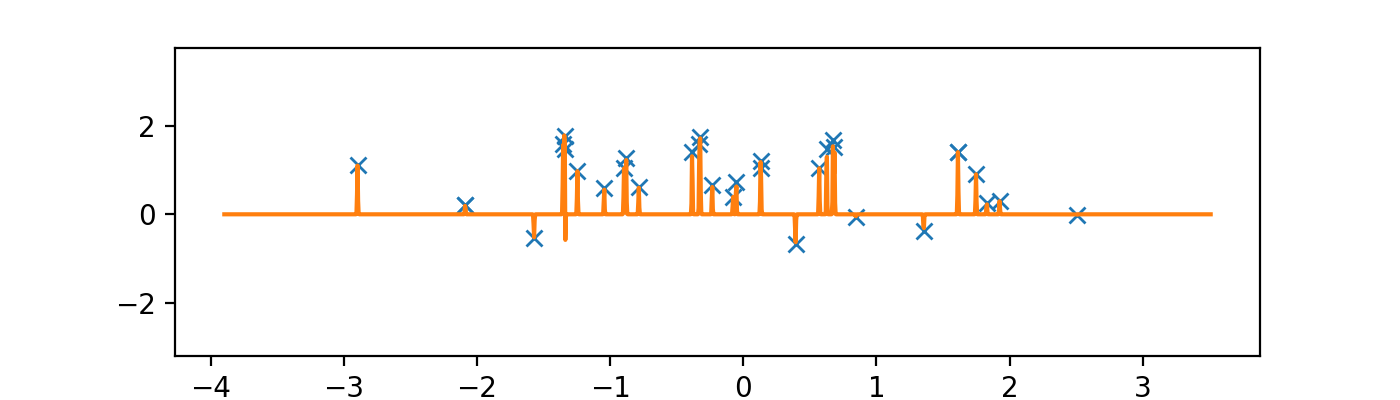
\includegraphics[width=\textwidth]{./figures/marginal_likelihood/overfit-novar.png}}
\onslide*<2>{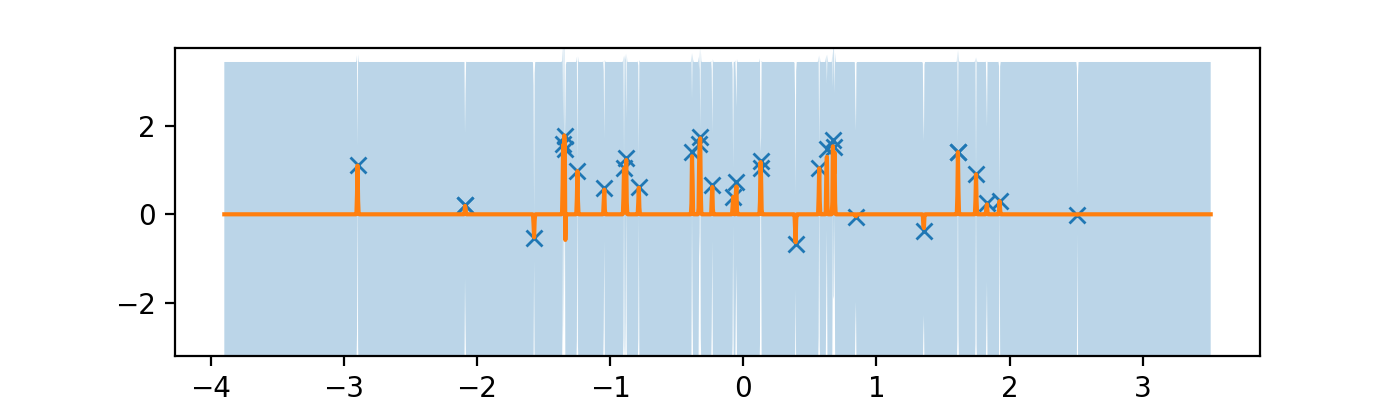
\includegraphics[width=\textwidth]{./figures/marginal_likelihood/overfit-var.png}}
\onslide*<3,4>{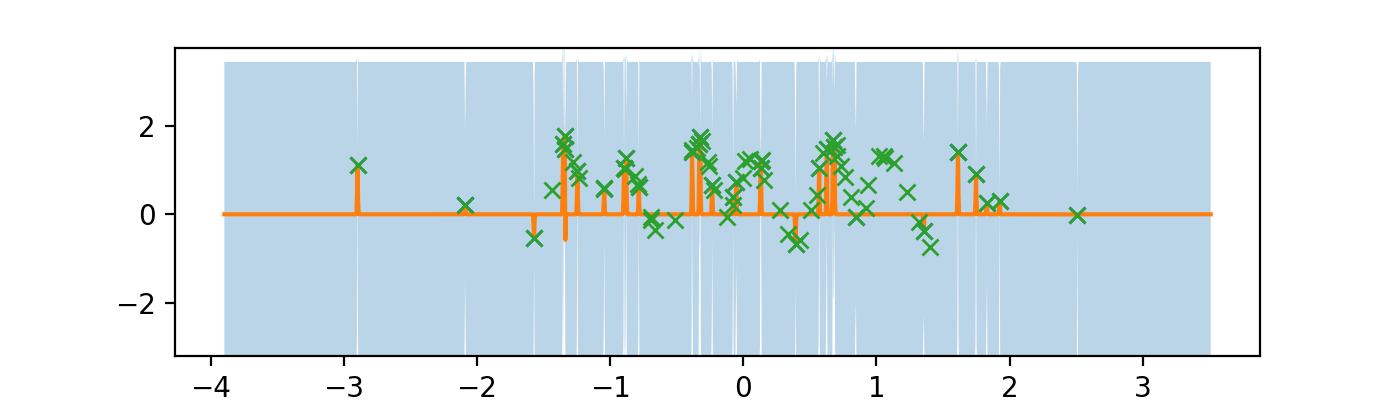
\includegraphics[width=\textwidth]{./figures/marginal_likelihood/overfit-var-testdata.png}}
\end{figure}
\pause
\pause
\pause
\begin{itemize}
\item Uncertainty by itself does not necessarily make predictions better, if the wrong model is chosen
\item Uncertainty does make predictions more cautious, which can be very useful!
\end{itemize}
\end{frame}





\begin{frame}{Marginal likelihood fixes things}
Instead, choose hyperparameters by maximising marginal likelihood:
\animategraphics[loop,controls,width=\linewidth]{20}{./figures/marginal_likelihood/animation_good_fit/good_fit-}{0}{101}
\vspace{-0.2cm}
\begin{center}
\tiny In above $\mathcal{L}$ is indicated by `datafit`, while `ELBO` indicates the marginal likelihood.
\end{center}
\begin{itemize}
  \item More sensible fit as the marginal likelihood rises
  \item Datafit gets worse!
\end{itemize}
\begin{center}
\Large Marginal likelihood trades off \\
\textbf{data fit} and \textbf{model complexity}.
\end{center}
\end{frame}


\begin{frame}{Why does marginal likelihood work?}
We have seen
\begin{itemize}
\item Minimising training error doesn't work
\item Uncertainty doesn't necessarily help, but does make us more cautious
\item Marginal likelihood seems to trade-off complexity and data fit
\end{itemize}

\begin{center}
\Large But \emph{why} does the marginal likelihood lead to models that generalise well?
\end{center}
\end{frame}



\begin{frame}{Marginal likelihood as incremental prediction}
  We can split the marginal likelihood up using the \emph{product rule}:
  \begin{align}
    p(\vy\given\theta, X) &= p(y_1|\theta, \vx_1) p(y_2|\theta, \vx_1, y_1, \vx_2) p(y_3|\theta, \{\vx_i, y_i\}_{i=1}^2, \vx_3) \dots \\
                          &= \prod_{n=1}^N p(y_n|\theta, \{\vx_i, y_i\}_{i=1}^{n-1}, \vx_n)
  \end{align}
\pause
Remember
\begin{align*}
p(y_n|\theta, \{\vx_i, y_i\}_{i=1}^{n-1}, \vx_n) = \int p(y_n | f(\vx_n)) p( f(\vx_n) \given \{\vx_i, y_i\}_{i=1}^{n-1}, \vx_n) \calcd{f(\vx_n)}
\end{align*}
i.e.~the predictive distribution of $y_n$ based on the posterior given all points up to $n-1$.
\end{frame}


\begin{frame}{Marginal likelihood as incremental prediction}
  We can split the marginal likelihood up using the \emph{product rule}:
  \begin{align}
    p(\vy\given\theta, X) &= p(y_1|\theta, \vx_1) p(y_2|\theta, \vx_1, y_1, \vx_2) p(y_3|\theta, \{\vx_i, y_i\}_{i=1}^2, \vx_3) \dots \\
                          &= \prod_{n=1}^N p(y_n|\theta, \{\vx_i, y_i\}_{i=1}^{n-1}, \vx_n)
  \end{align}

  \vspace{0.5cm}

  \begin{itemize}
  \item The marginal likelihood measures how well previous training points predict the next one
  \item If it continuously predicted well on all $N$ points previously, it probably will do well next time
  \end{itemize}
\end{frame}


\begin{frame}{Marginal likelihood computation in action}
\animategraphics[loop,controls,width=\linewidth]{1.5}{./figures/marginal_likelihood/animation_incremental/short_lengthscale/fig}{0}{45}
\end{frame}


\begin{frame}{Marginal likelihood computation in action}
\animategraphics[loop,controls,width=\linewidth]{1.5}{./figures/marginal_likelihood/animation_incremental/long_lengthscale/fig}{0}{45}
\end{frame}


\begin{frame}{Marginal likelihood computation in action}
\animategraphics[loop,controls,width=\linewidth]{1.5}{./figures/marginal_likelihood/animation_incremental/opt_lengthscale/fig}{0}{45}
\end{frame}


\begin{frame}{Marginal likelihood evolution}
\begin{figure}[T]
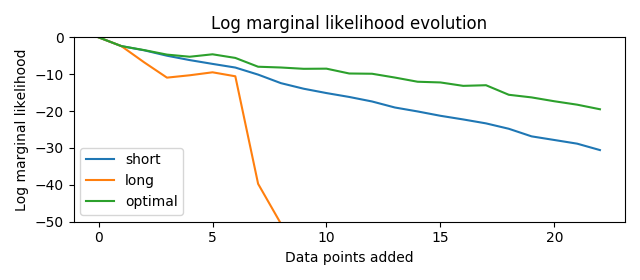
\includegraphics[width=\textwidth]{./figures/marginal_likelihood/marglik-evolution.png}
\end{figure}
\vspace{-0.5cm}
\begin{itemize}
\item \textbf{Short} lengthscale consistently \emph{over-estimates variance}, so \emph{can't get a high density} even with the observation in the error bars 
\item \textbf{Long lengthscale} consistently \emph{under-estimates variance}, so gets a low density because the \emph{observations are outside error bars}
\item Optimal lengthscale \emph{trades off} these behaviours...\pause~well.
\end{itemize}
\end{frame}


\begin{frame}{Generalisation}
\begin{itemize}
\item A model with a high marginal likelihood is likely to \emph{generalise} well.
\item Its inductive bias has correctly predicted the next training point throughout the entire training set.
\item Marginal likelihoods are also related to \emph{generalisation error bounds}.
\end{itemize}
\pause
Generalisation error bounds state things like:
``With high probability, the error for method X on a test set will not be larger than Y''

\vspace{0.3cm}

PAC-Bayesian Theory Meets Bayesian Inference \citep{germain2016pac}
\end{frame}


\begin{frame}{Marginal likelihood as a prior probability}
A complementary view

\begin{itemize}
\item Marginal likelihood is the probability of the data under the prior.
\begin{align}
p(\vy|\theta, X) = \int p(\vy\given f(X), \theta) p(f(X)\given \theta) \calcd{f(X)}
\end{align}
\item For zero-mean GP regression models it has the explicit form:
\begin{align}
\log p(\vy|\theta, X) &= \log \NormDist{\vy; 0, \mathbf{K} + \sigma^2 \mathbf{I}} \\
&= -\frac{N}{2}\log 2\pi - \underbrace{\frac{1}{2}\log \detbar{\mathbf{K} +\sigma^2 \mathbf{I}}}_{\text{Complexity penalty}} - \underbrace{\frac{1}{2} \vy\transpose\left(\mathbf{K} + \sigma^2\mathbf{I}\right)\inv\vy}_{\text{Data fit}} \nonumber
\end{align}
\end{itemize}
\end{frame}


\begin{frame}{Complexity penalty and data fit}
\begin{align}
\log p(\vy|\theta, X) &= -\frac{N}{2}\log 2\pi - \underbrace{\frac{1}{2}\log \detbar{\mathbf{K} +\sigma^2 \mathbf{I}}}_{\text{Complexity penalty}} - \underbrace{\frac{1}{2} \vy\transpose\left(\mathbf{K} + \sigma^2\mathbf{I}\right)\inv\vy}_{\text{Data fit}}
\end{align}

\begin{itemize}
\item Determinant is product of eigenvalues (variances) of the covariance matrix -- the volume of the prior
\item Quadratic term measures whether the observation $\vy$ is within the variation allowed by the prior -- by lining $\vy$ up with the eigenvectors of the covariance
\end{itemize}

\end{frame}


\begin{frame}{Simple and complex models}
Probabilities have to normalise to 1, so a model \textbf{cannot} both
\begin{itemize}
\item be flexible enough to fit many datasets, and
\item make specific predictions after only a small amount of data.
\end{itemize}
\begin{figure}[T]
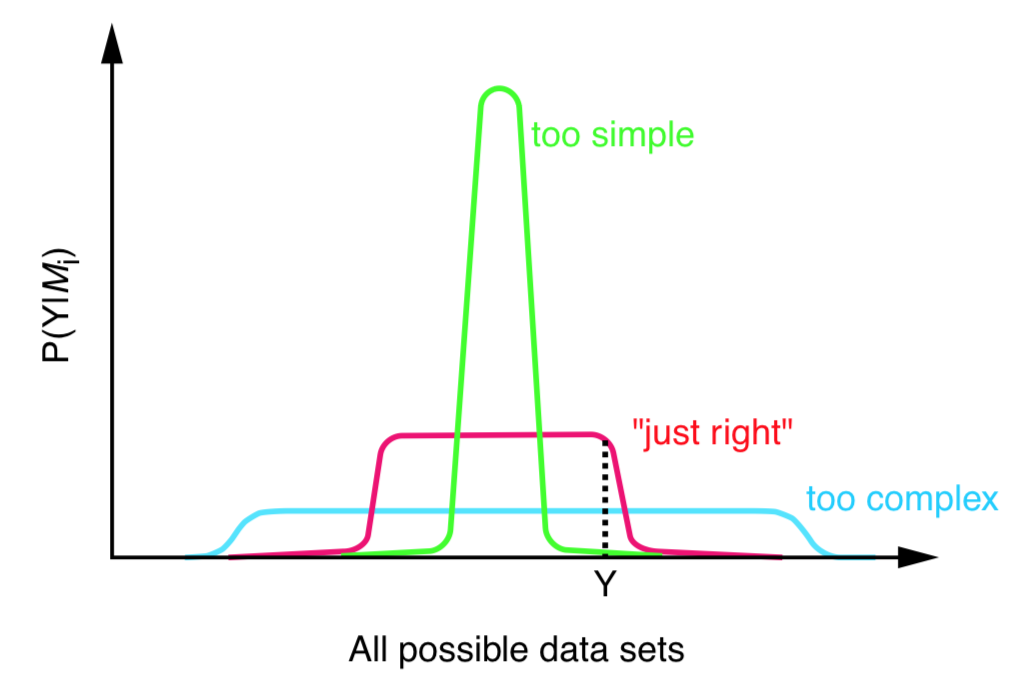
\includegraphics[width=0.5\textwidth]{./figures/marginal_likelihood/occam.png}
\end{figure}
\vspace{-0.7cm}
\begin{center}
\tiny From ``Occam's Razor'' -- Rasmussen \& Ghahramani (2000)
\end{center}
\begin{itemize}
\item Complex / flexible models spread their probability over many possible explanations of the data
\end{itemize}
\end{frame}

\begin{frame}{Occam's razor}
  \begin{center}
    \textit{``Entities are not to be multiplied without necessity''}\\
    or\\
    \textit{The simplest solution is most likely the right one} \\

    \vspace{1.0cm} \pause

    {\Large The marginal likelihood prefers the simplest model that still fits the data.}
  \end{center}
\pause
The marginal likelihood
\begin{itemize}
\item automatically penalises complex models, as the old adage states
\item comes from a principle as simple as representing your belief using probability
\item is automatically applied if you use Bayes' rule properly
\end{itemize}
\end{frame}


\begin{frame}{Marginal likelihood in action}
\animategraphics[loop,controls,width=\linewidth]{20}{./figures/marginal_likelihood/animation_periodic_fit/periodic_fit-}{0}{101}
\pause
\begin{itemize}
  \item Marginal likelihood learns \emph{how} to generalise
not just to fit the data.
  \item We chose the prior: $f(\vx) = \theta_sf_\text{smooth}(\vx) + \theta_pf_{\text{periodic}}(\vx)$, with smooth and periodic GP priors respectively.
  \item Amount of periodicity vs smoothness is automatically chosen by selecting hyperparameters $\theta_s, \theta_p$.
\end{itemize}
\end{frame}


\begin{frame}{Marginal likelihood in action}
\animategraphics[loop,controls,width=\linewidth]{1.5}{./figures/marginal_likelihood/animation_incremental/periodic/fig}{2}{45}
\end{frame}


\begin{frame}{Further reading}
\begin{itemize}
\item \nocite{itila} David~J.C.~MacKay. \textit{Information Theory, Inference, and Learning Algorithms}, chapter 28.
\end{itemize}
\end{frame}




%%%%%%%%%%%%%%%%%%%%%%%%%%%%%%%%%%%%%%%%%
% REFERENCES
%%%%%%%%%%%%%%%%%%%%%%%%%%%%%%%%%%%%%%%%%
\begin{frame}[t,allowframebreaks]
\frametitle{References}
\linespread{1.0}
\tiny
\bibliographystyle{abbrv}
\bibliography{../includes/pi-literature.bib}
\end{frame}



\end{document}
%%% Local Variables: 
%%% mode: latex
%%% TeX-master: t
%%% End: 
